% 5. Einleitung

\chapter{Results and Discussion}

When applying all corrections, presented in chapter~\ref{chap:fvz}, to the measured zenith angles $z_b$ one obtains the true zenith angles $z$ as presented in Fig.~\ref{fig:zenith}. The zenit angles are given as a function of universal time (UT) in hours, at which the individual measurements have been taken. 
From the decreasing value of $z$ with time, one can deduce that all measurements have been taken before noon, since a rising sun coencides with decreasing zenith angles. \\ The error bars in Fig.~\ref{fig:zenith} correspond to the error of the zenith angle $z$ and are, in this representation, barely visible. The fact that some of the data points deviate significantly from the expected errors can be attributed to the fact that the central crosshair in the theodolite's scope was reported to be mistaken with one of the outer crosshairs for some of the measurements. Additional contributions to the error might come from the fact that the theodolite is not perfectly leveled, giving an unknown error.\\


\begin{figure}[]
    \centering
    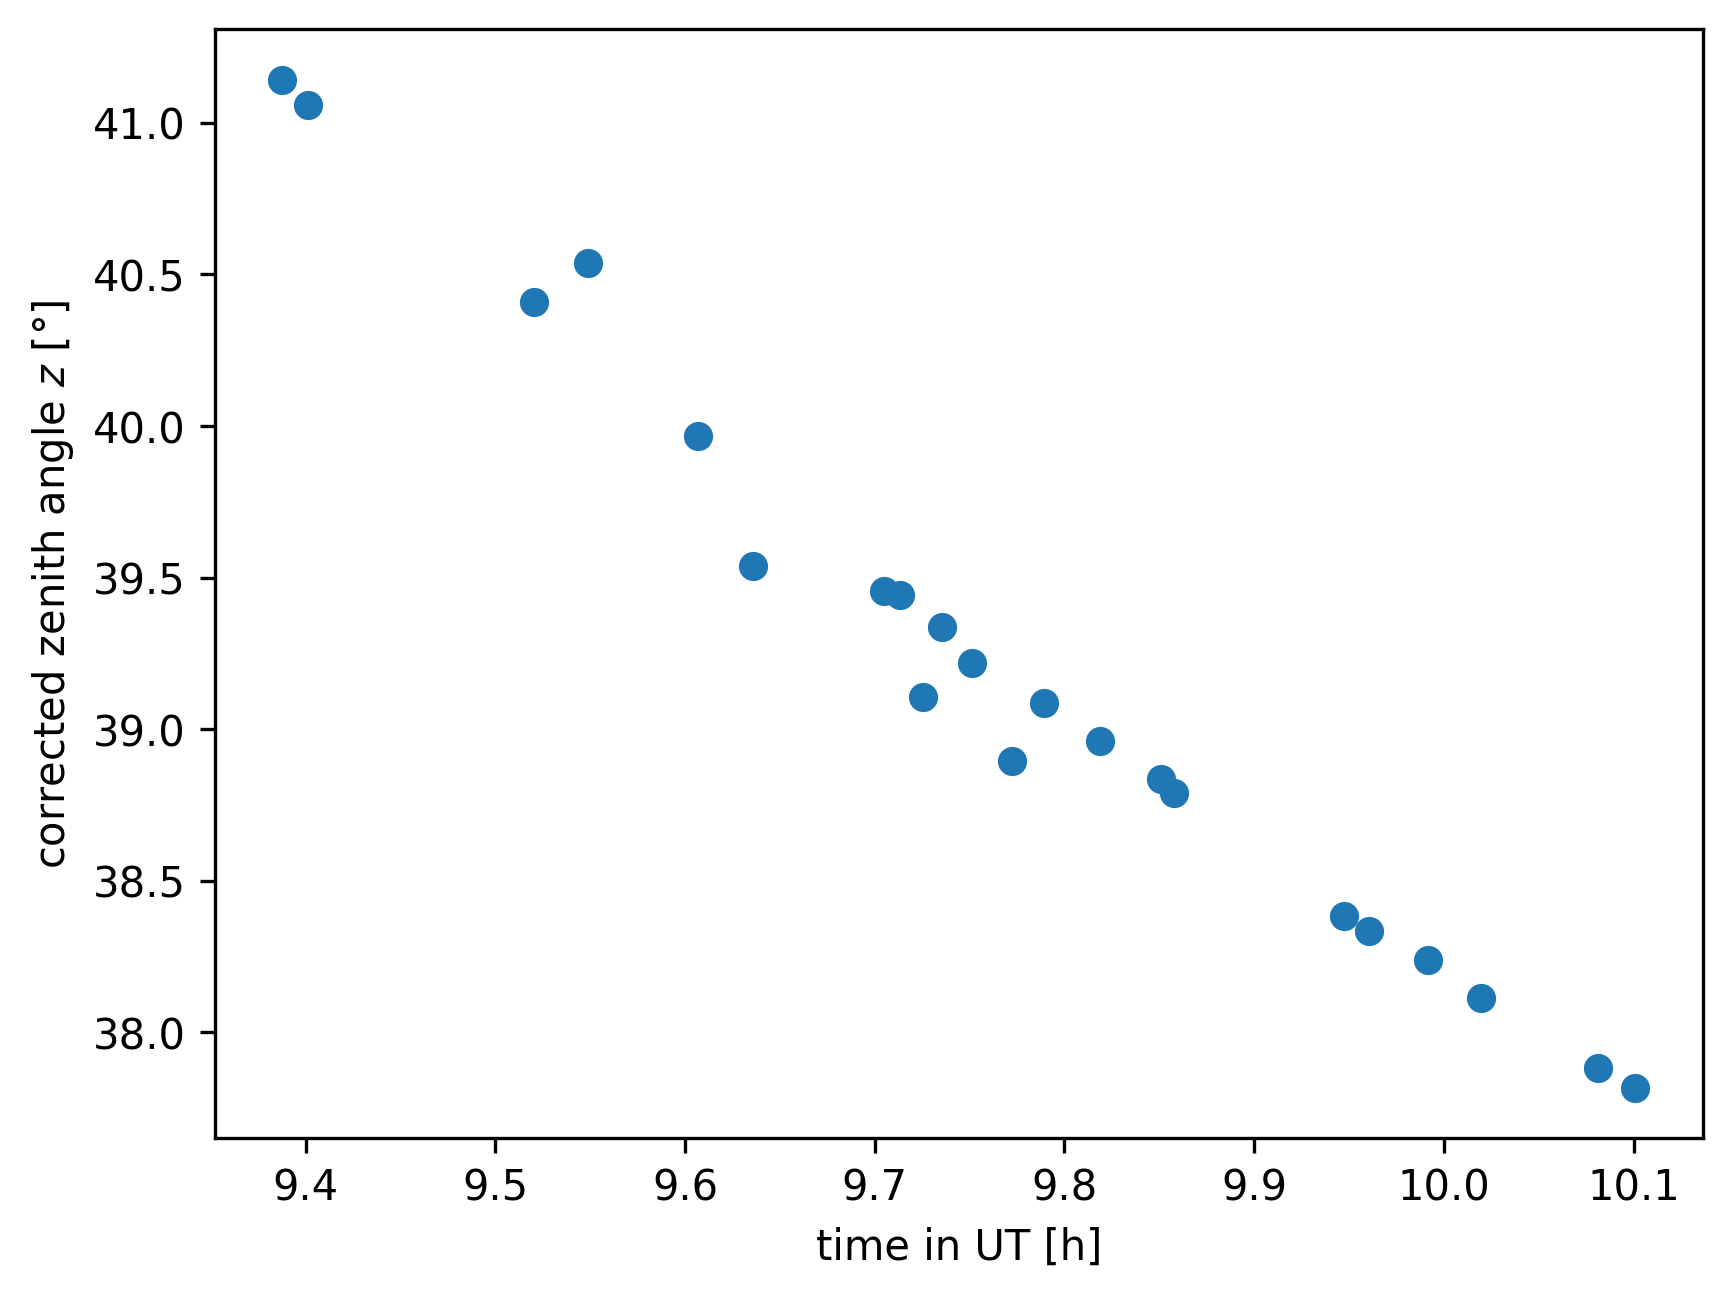
\includegraphics[width=0.9\textwidth]{05-Fazit/zenith_angle_plot.png}
    \caption{Corrected zenith angle $z$, obtained according to Eq.~(\ref{eq:zenith_angle_corrections}), as function of measurement time in UT.}
    \label{fig:zenith}
\end{figure}

\label{chap:fazit}

From the corrected zenith angles $z$ the geographical latitude $b$ can be calculated using Eq.~\ref{eq:latitude}. Here three possible solutions are given, which again depend on the location on earth, i.e. $b$, and the time of observation (contained in $Y$). In fact, there are four solution for $b$, corresponding to the northern and southern hemisphere as well as summer and winter seasons. When considering that summer and winter are reversed on northern and southern hemispheres, one can explain the fact that two of these equations are in fact identicla (question d).\\
We find that $(b+Y)>\pi/2$, when using the GPS determined latitude $b=52^\circ 27' 24''$N, thus the first solution in Eq.~(\ref{eq:latitude}) has to be applied to our measurement data. The obtained latitude for each measurement is presented in Fig.~\ref{fig:latitude}.

\begin{figure}[]
    \centering
    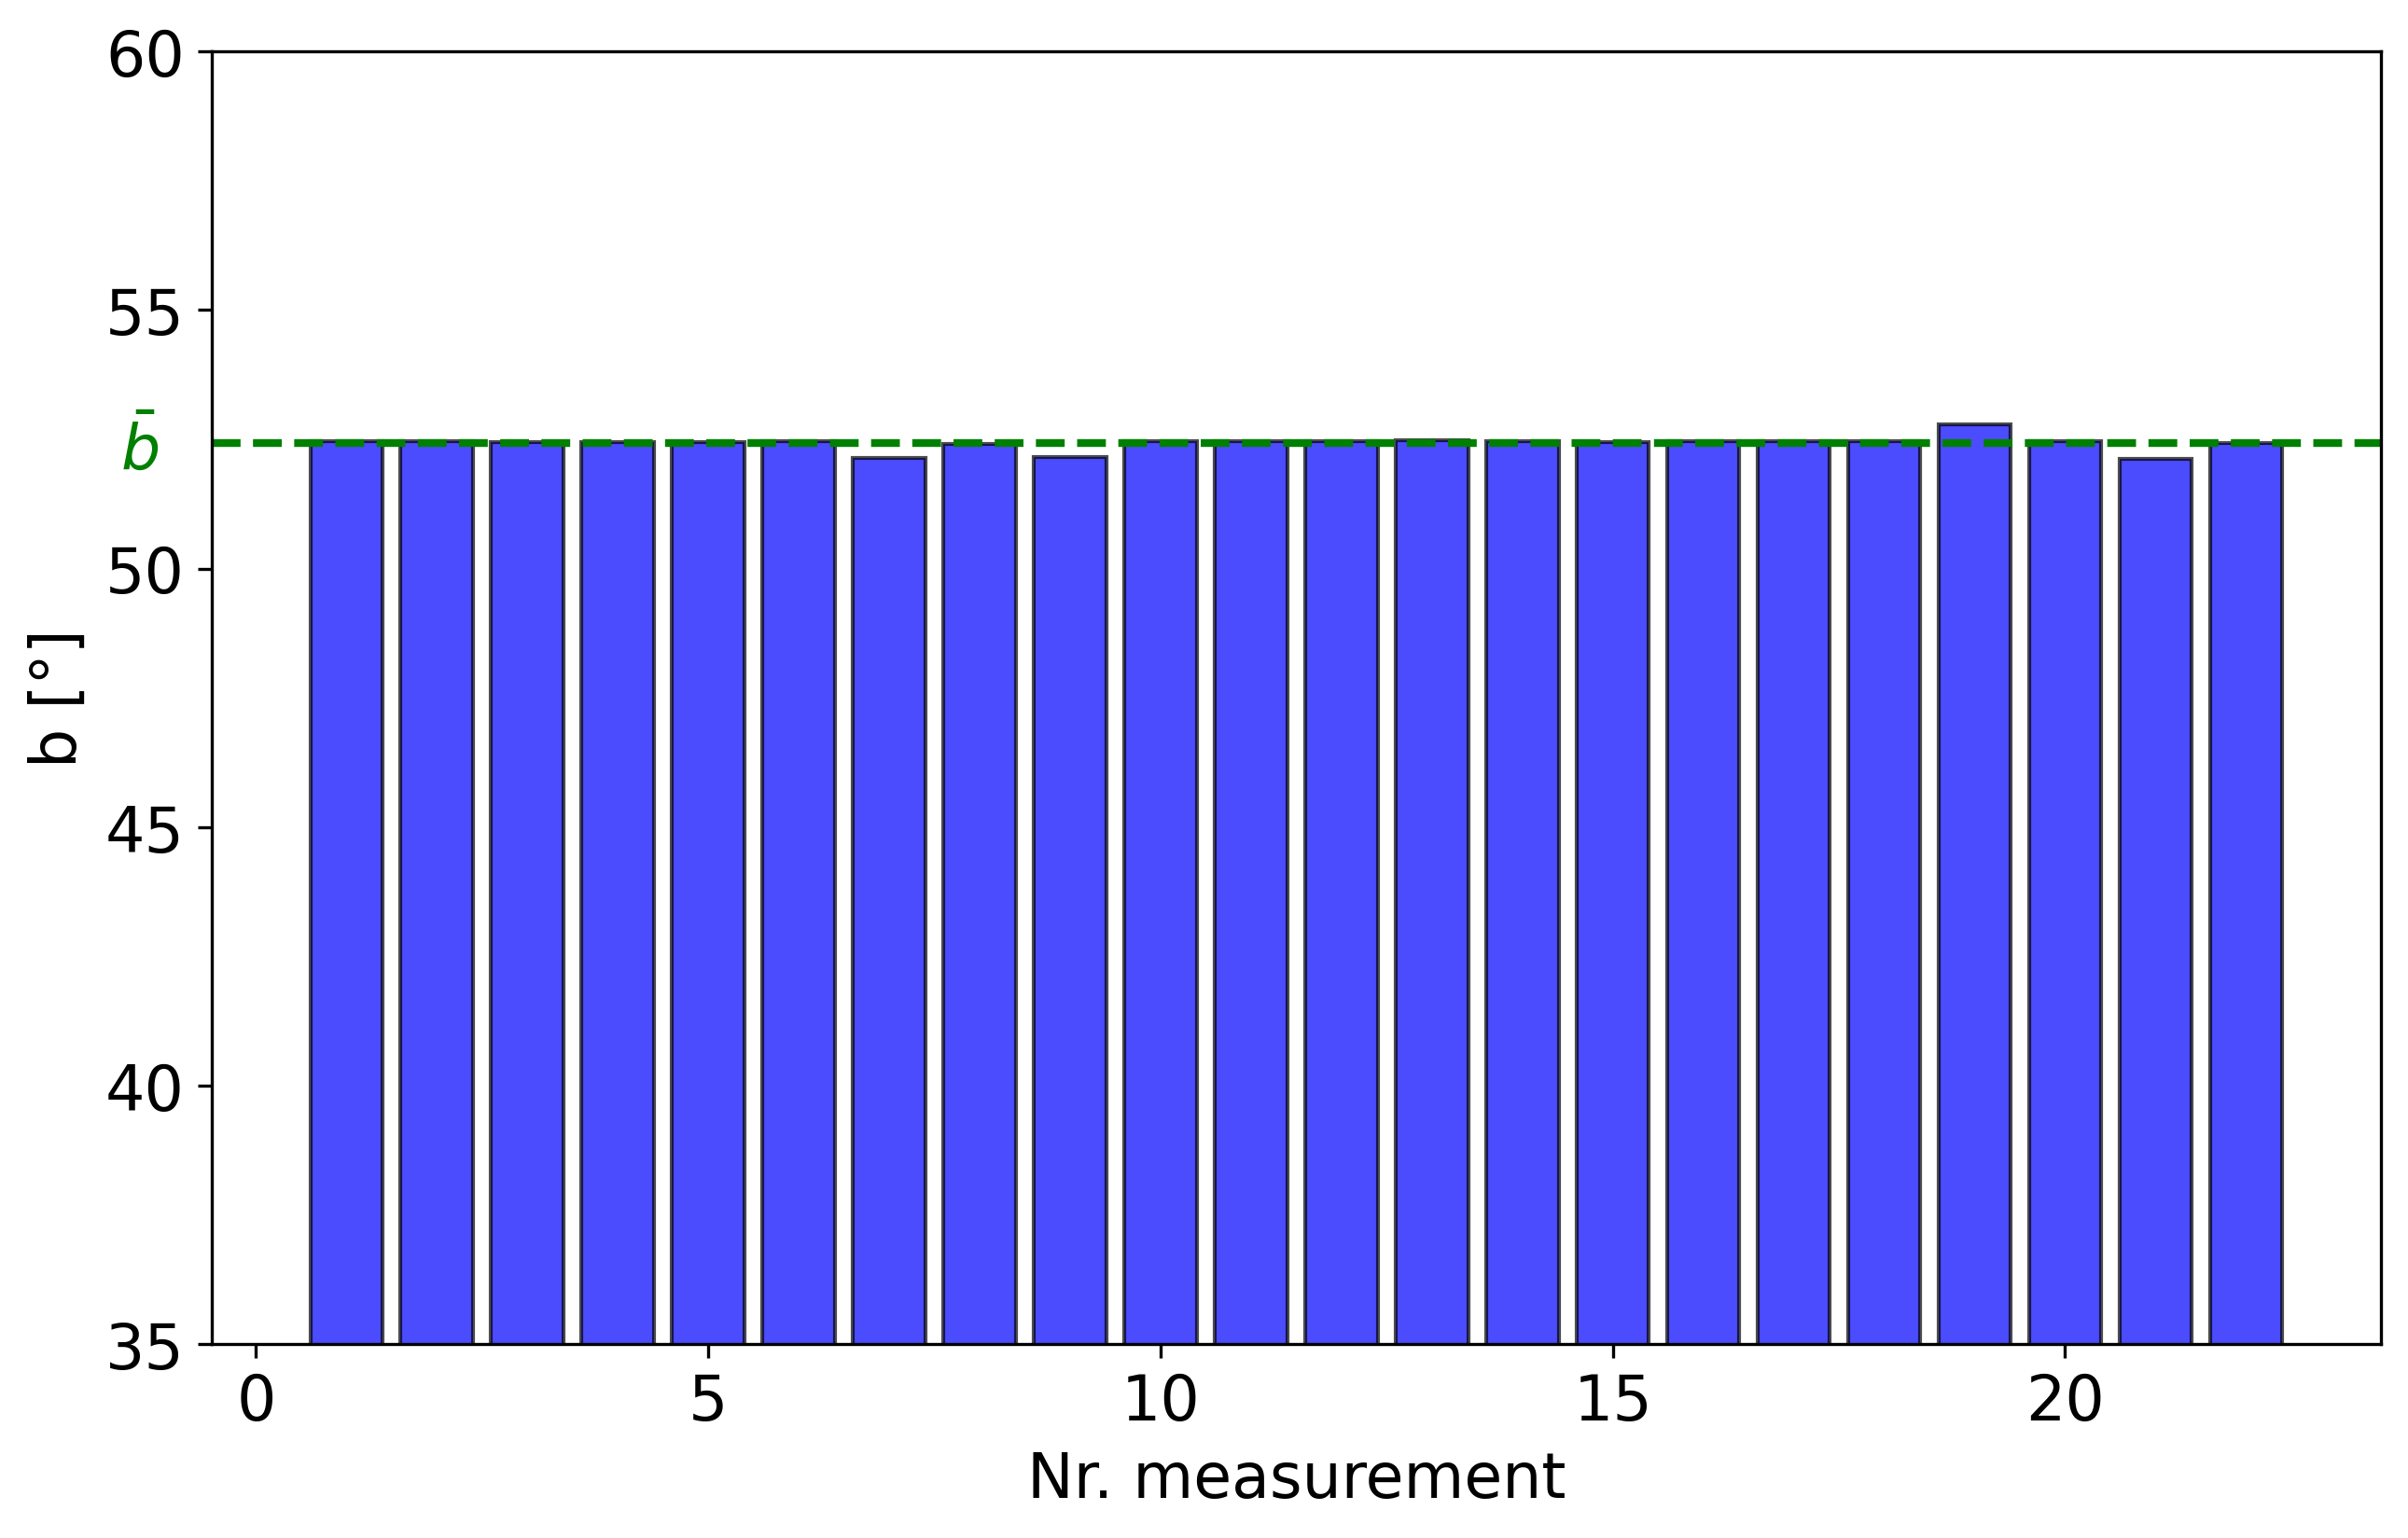
\includegraphics[width=0.9\textwidth]{05-Fazit/histogram.png}
    \caption{Geographical latitude $b$, obtained according to Eq.~(\ref{eq:latitude}), as function of measurement number. Error bars correspond to the individual values of latitude and $\bar b$ gives the average latitude.}
    \label{fig:latitude}
\end{figure}

When computing the average latitude, we determine a value of $\bar b =52.428 \pm 0.019$ or $\bar b = 52^\circ 25' 40'' \pm 1' 9''$. A comparison to the true latitude of $b=52^\circ 27' 24''$, determined via GPS, shows a good agreement between both valuse. However, the calculated value does not include the GPS value within the determined error. 


% Text